% \documentclass{beamer}
\documentclass{standalone}
\usepackage[utf8]{inputenc}
\usepackage{montserrat}
\usepackage{tikz}
\usetikzlibrary{positioning}
\usetikzlibrary{arrows.meta}
\usetikzlibrary{through}
\usetikzlibrary{backgrounds}
\setlength\parindent{0pt}

% \beamertemplatenavigationsymbolsempty

\renewcommand{\familydefault}{\sfdefault}

\begin{document}

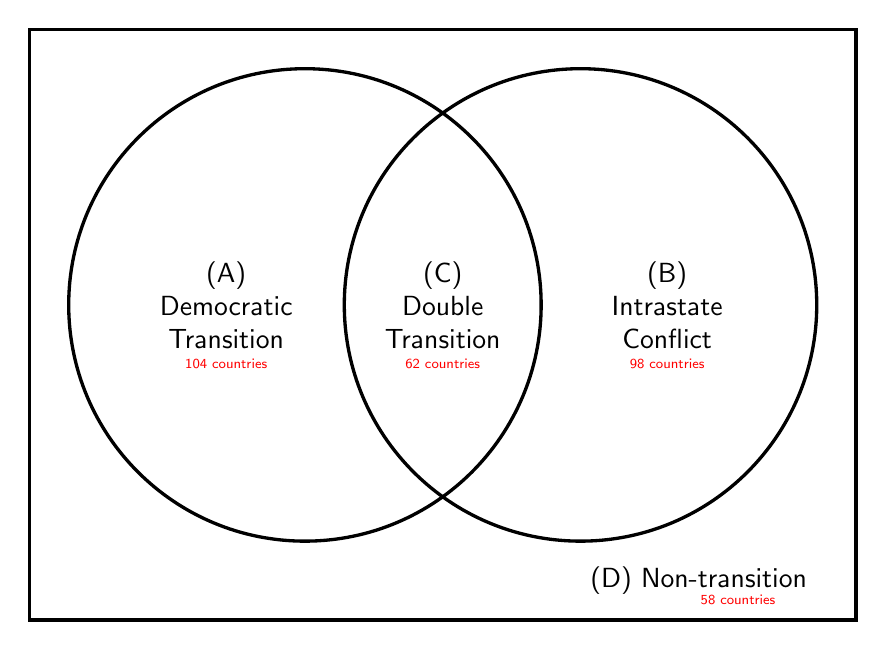
\begin{tikzpicture}[very thick, scale=1, black, align=center]
  \coordinate (O) at (0,0);
  \draw (0,0) rectangle + (10.5,7.5);
  \draw (3.5,4) circle [radius=3];
  \draw (7,4) circle [radius=3];
  \node at (2.5,4) {(A)\\Democratic\\Transition};
  \node[red, font=\tiny] at (2.5,3.25) {104 countries};
  \node at (5.25,4) {(C)\\Double\\Transition};
  \node[red, font=\tiny] at (5.25,3.25) {62 countries};
  \node at (8.1,4) {(B)\\Intrastate\\Conflict};
  \node[red, font=\tiny] at (8.1,3.25) {98 countries};
  \node at (8.5,0.5) {(D) Non-transition};
  \node[red, font=\tiny] at (9,0.25) {58 countries};
\end{tikzpicture}

\end{document}